\documentclass[letter,10.5pt]{article}
\usepackage{graphicx}
\usepackage{array}
\usepackage{booktabs}
\usepackage{amsfonts,amssymb,amsmath,amsthm}
\usepackage{boxedminipage}
\usepackage{bm}
\usepackage{color}
\usepackage{url}
\usepackage{enumerate}

\newcommand{\rmnum}[1]{\romannumeral #1}
\newcommand{\Rmnum}[1]{\MakeUppercase{\romannumeral #1}}
\newcommand{\prob}{\mathbb{P}}
\newcommand{\E}{\mathbb{E}}
\newcommand{\Normal}{\mathsf{N}}
\newcommand{\iid}{\stackrel{\text{iid}}{\sim}}
\newcommand{\R}{\mathbb{R}}

\numberwithin{equation}{subsection}

% grouping operators
\newcommand{\brac}[1]{\left[#1\right]}
\newcommand{\set}[1]{\left\{#1\right\}}
\newcommand{\abs}[1]{\left\lvert #1 \right\rvert}
\newcommand{\paren}[1]{\left(#1\right)}
\newcommand{\norm}[1]{\left\|#1\right\|}


\setlength{\textwidth}{150mm}
\setlength{\textheight}{230mm}
\setlength{\headheight}{-1.5cm}
\setlength{\topmargin}{-0.1cm}
\setlength{\oddsidemargin}{0cm}
\setlength{\evensidemargin}{0cm}
\setlength{\parskip}{1mm}
\setlength{\unitlength}{1mm}
\setlength{\parindent}{2.06em}
\pagestyle{plain}

\title{\textbf{STAT 406 Lab 4 Handout}}
\author{Jun Guo}
\date{\today}
\begin{document}
\begin{center}
\large
\textbf{STAT 406 Lab 4, 10/06/2015}
\end{center}\vspace*{5mm}


\noindent
% ---------------------------------
\textbf{1. Generate Random Variable}
% ---------------------------------

\normalsize
\noindent
We learned from lecture that random variables from a particular distribution can be gen- erated from uniform random variables by inverting their cumulative distribution function (cdf). That is, if you create samples $U_1, \cdots , U_n$ from $Uniform(0, 1)$ distribution and compute $F^{-1}(U_1), \cdots , F^{-1}(U_n)$, then what you get is samples from a distribution with cdf $F$ . Using this property, we'll generate exponential random variables and gamma random variables.

\noindent \textbf{(a)} The Exponential$(\lambda)$ distribution has cdf:
\begin{equation*}
F(x) = 1 - e^{-\lambda x}, \lambda > 0
\end{equation*}
Using $runif$ function, generate 100 samples from $Exponential(3)$ distribution using the inversion method. Graph the density histogram for the sample with the true density superimposed for comparison.\\
\begin{boxedminipage}{\textwidth}
\scriptsize
\begin{verbatim}
n = 100
lambda = 3
x = -(1/lambda)*log(runif(n))
hist(x, prob = TRUE)
y = seq(0,10,length = 1000)
lines(y,dexp(y,3))
\end{verbatim}
\end{boxedminipage}
\begin{center}
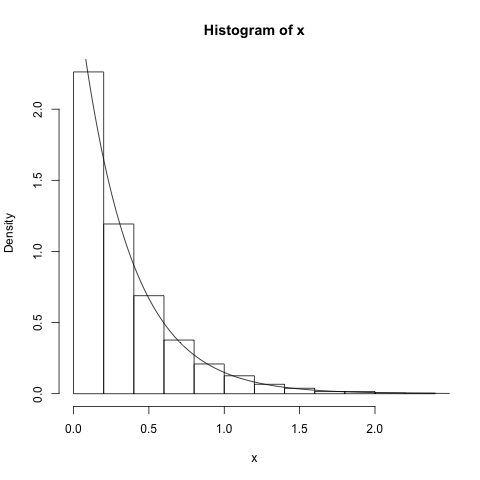
\includegraphics[scale=0.3]{1a.png}
\end{center}
\noindent
\textbf{(b)} $Gamma(k, \theta)~,~k>0,~\theta>0$ distribution has density:
$$f(x) = \frac{\theta^k}{(k-1)!}x^{k-1}e^{-\theta x}$$
where $k~and~\theta$ are shape and rate parameters. What are $k~and~\theta$ for $Exponential(\lambda)$ distribution in terms of Gamma distribution?

Gamma distribution also has the property that if $X \sim Gamma(a, \theta)$ and $Y \sim Gamma(b, \theta)$, and $X$ and $Y$ are independent, then
$$X+Y \sim Gamma(a+b,\theta).$$ Using this property, create 10 samples from Gamma(5, 3) distribution.

\begin{boxedminipage}{\textwidth}
\scriptsize
\begin{verbatim}
n = 10
k = 5
lambda = 3
x = matrix(-(1/lambda)*log(runif(n*k)), ncol=k)
g = apply(x, 1, sum)
\end{verbatim}
\end{boxedminipage}

\noindent
\textbf{(c)} Take an n-sample from the Gamma(5, 3) using your algorithm from part (b), with $n = 10, 20, 50, 100, 200, 1000.$

\begin{boxedminipage}{\textwidth}
\scriptsize
\begin{verbatim}
n = c(10, 20, 50, 100, 200, 1000)
g = list()
k = 5
lambda = 3
g = lapply(n, function(i) matrix(-(1/lambda)*log(runif(i*k)), ncol=k))
class(g) #to see what is the data structure used for g
sapply(g, dim) #check the dimension of each matrix in g
## the following will get the gamma random numbers of different sizes n. ##
gamma = lapply(g, function(M) matrix(-(1/lambda)*log(runif(i*k)), ncol=k)) 
class(gamma) #to see what is the data structure
sapply(gamma, length) #check the dimension of each vector in g
\end{verbatim}
\end{boxedminipage}

\noindent
\text{(d)} Now, use R function \textbf{density} to obtain an estimate of the underlying density. Show how the estimate gets better as n increases, and graph the estimated densities and the true density superimposed for comparison. 

\begin{boxedminipage}{\textwidth}
\scriptsize
\begin{verbatim}
#continue with gamma from the output of part (c)
grid = 1000
y = seq(0,10,length = grid)
plot(0,xlim=c(0,10),ylim=c(0,1),xlab="x",ylab="Density",main="Gamma density estimation", type='n')
par(mfrow=c(2,3))
for(i in 1:6){
    di = density(gamma[[i]],from=0,to=10, n = grid, bw=0.2)
    plot(di, xlim=c(0,10), ylim=c(0,1), axes=F, col=rainbow(6)[i], lwd = 2, main="Gamma density estimation")
    lines(y,dgamma(y,5,3), col = 'orange', lty = 3, lwd = 2)
}

names(di) #check to see what are in the density estimator output di, notice di$x and di$y
##multiple plot in R : http://cran.r-project.org/doc/contrib/Lemon-kickstart/kr_addat.html
\end{verbatim}
\end{boxedminipage}
\begin{center}
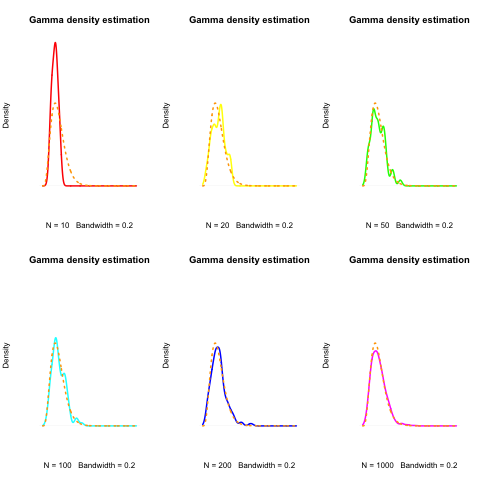
\includegraphics[scale=0.4]{1d23.png}
\end{center}

\noindent
\large
% ---------------------------------
\textbf{2. More of LLN - Empirical Distribution Functions}
% ---------------------------------
\normalsize

Write a function which calculates the empirical distribution function of $X_1,\cdots,X_n\stackrel{\text{iid}}{\sim}N(0,1)$. The empirical distribution function is defined as
\begin{equation*}
\Phi_m(x) = \frac{1}{n}\sum_{i=1}^nI(X_i\leq x)
\end{equation*}
where $I(X\leq x)$ is an indicator function, taking value 1 if $X\leq x$ and 0 otherwise. Plot this function for $x\in[-4,4]$. Let $m=5,50,500$ respectively and plot everything on the same figure, with the true Normal cdf superimposed for comparison. 

\begin{boxedminipage}{\textwidth}
\scriptsize
\begin{verbatim}
Phi.m = function(m,xseq){
	# xseq can be either a scalar or a vector
	X = rnorm(m)
	Phi.m.x = sapply(xseq,function(x){mean(X<x)})
	return(Phi.n.x)
}

m = c(5,50,500)
xseq = seq(-4,4,by=0.01)
plot(0,xlim=c(-4,4),ylim=c(0,1),xlab="x",ylab="Phi.m(x)",main="Empirical CDF", type='n')
for (i in 1:length(m)){
	par(new=T)
	plot(xseq,Phi.n(m[i],xseq),col=i,axes=F,type="l",xlim=c(-4,4),ylim=c(0,1),xlab="",ylab="")
}
lines(xseq,pnorm(xseq,mean=0,sd=1),col="blue",lty=3,lwd=2)
legend("topleft",legend=paste(m,'points'),col=1:length(m),lty=1)
\end{verbatim}
\end{boxedminipage}
\begin{center}
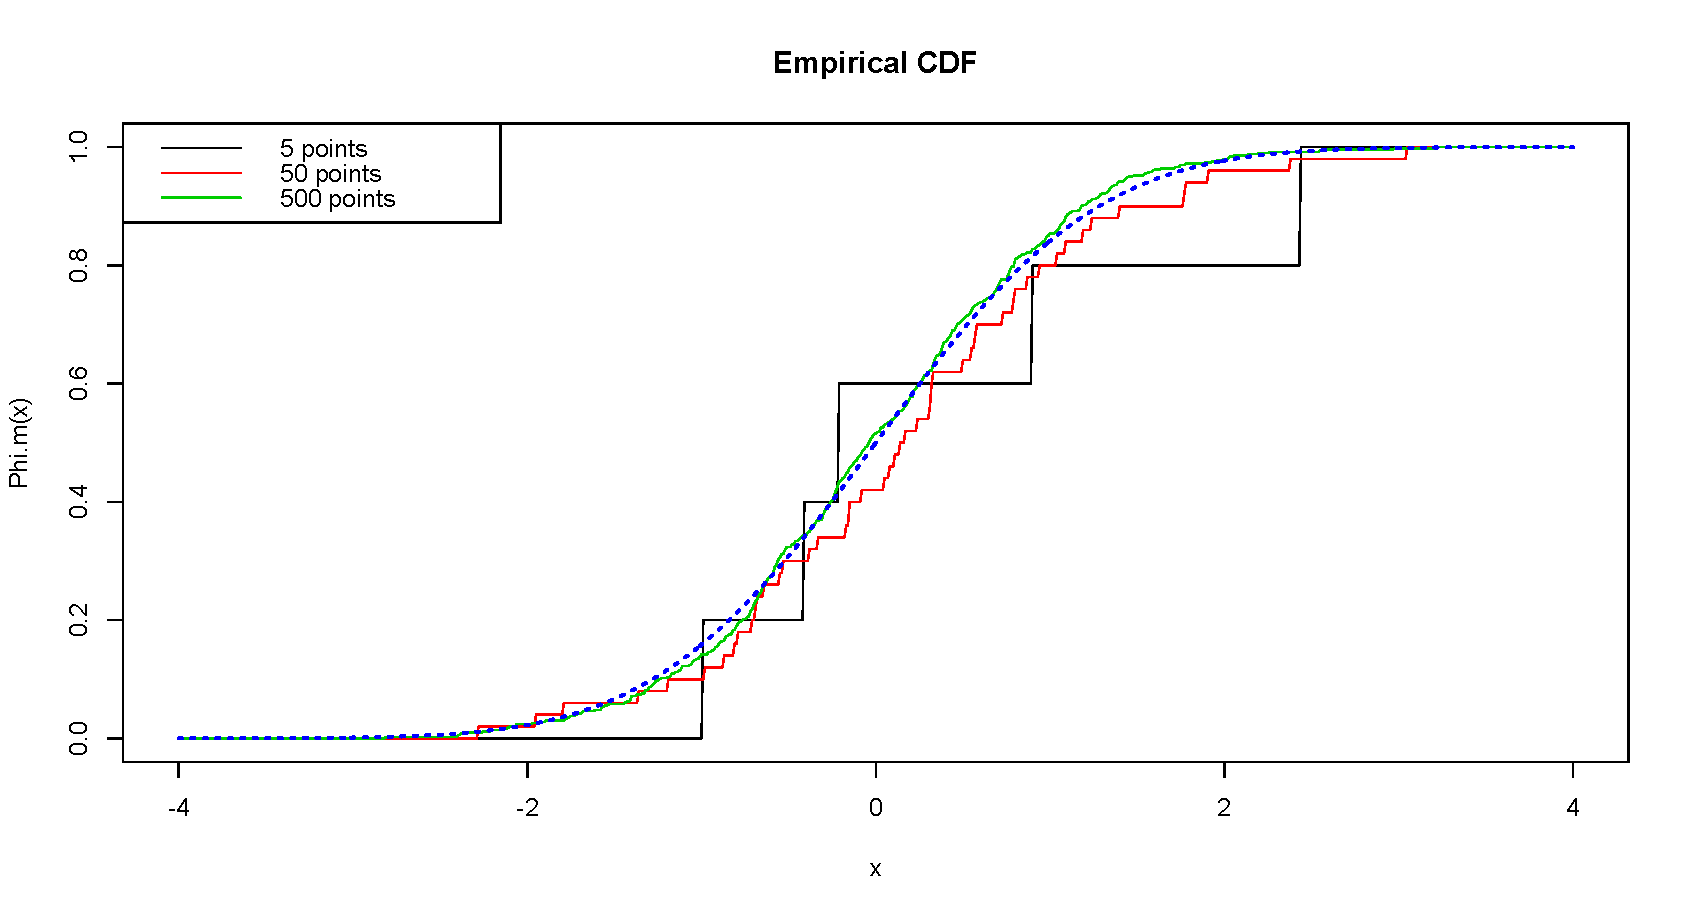
\includegraphics[scale=0.4]{2cdf.pdf}
\end{center}


\end{document}